%========================================================
% CHAPTER 1 — Physical and Mathematical Framework
%========================================================

This chapter introduces the physical representation and mathematical tools used
throughout the thesis to describe polarization-entangled photon pairs and their
evolution through optical-fiber channels. The treatment is formulated within the
density-operator framework of quantum information theory, which provides a common
description for pure states, statistical mixtures, local measurements, and noisy
quantum evolution~\cite{nielsen_chuang_qcqi}.

The chapter first defines the bipartite polarization system and the reference Bell
state. The density-operator and reduced-state formalisms are then introduced,
followed by the description of two-photon polarization measurements and
correlations. The main quantities used to characterize the propagated quantum
state are subsequently defined, with particular attention to purity, fidelity,
concurrence, tangle, and entanglement of formation.

Finally, the chapter introduces the BBM92 entanglement-based quantum key
distribution protocol as the main operational reference of this work. Its
measurement scheme and principal quantities of interest, including the quantum
bit error rate and secret-key conditions, are presented in order to establish the
connection between the quality of the distributed entangled state and its
suitability for secure quantum communication. This provides the operational basis
for interpreting the fiber-propagation models and numerical results developed in
the following chapters.

%========================================================
% SECTION 1.1 — Bipartite Polarization System
%========================================================

\section{Bipartite Polarization System}
\label{sec:bipartite_polarization_system}

The physical system considered in this work consists of a pair of
polarization-entangled photons propagating along two spatially separated optical
paths, denoted by \(A\) and \(B\). In the experimental configuration considered
later in this thesis, the photon pairs are produced through high-fidelity 
spontaneous parametric down-conversion (SPDC).

The quantum information carried by each photon is encoded in its polarization
degree of freedom. Horizontal and vertical polarization are identified with the
computational basis according to

\begin{equation}
|H\rangle \equiv |0\rangle,
\qquad
|V\rangle \equiv |1\rangle.
\label{eq:polarization_computational_encoding}
\end{equation}

Each photon therefore defines a two-dimensional Hilbert space,

\begin{equation}
\mathcal{H}_A \simeq \mathbb{C}^{2},
\qquad
\mathcal{H}_B \simeq \mathbb{C}^{2}.
\end{equation}

The Bloch sphere provides a geometric representation of the state of a single
qubit, as illustrated in Fig.~\ref{fig:polarization_bloch_sphere}. Pure states
are represented by points on the surface of the sphere, while the polar angle and
azimuthal angle determine the relative amplitudes and phase of the two basis-state
components. Coherent superpositions occupy the remaining points on the sphere,
with equal-weight superpositions lying on the equator.

\begin{figure}[t]
    \centering
    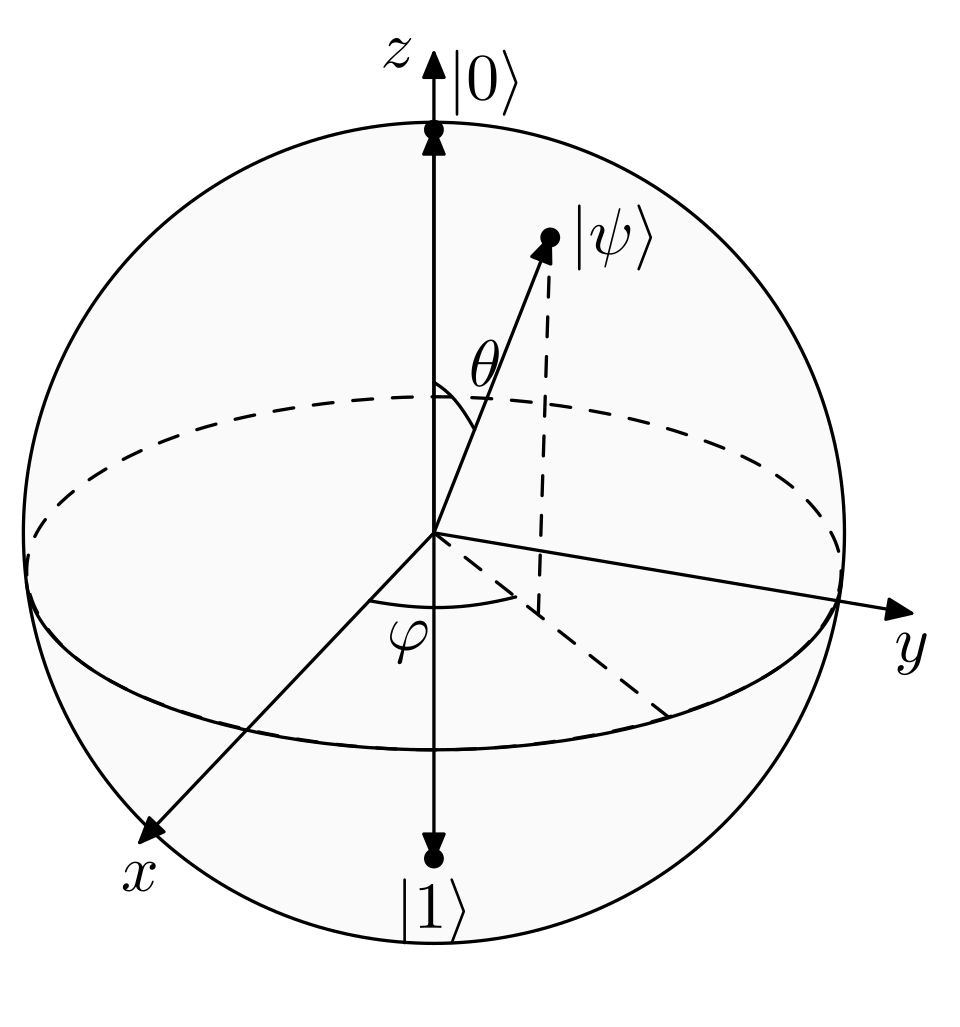
\includegraphics[
        width=0.42\textwidth
    ]{figures/theory/bloch_sphere_representation.png}
    \caption{
    Bloch-sphere representation of a single polarization qubit.
    The horizontal and vertical polarization states correspond to
    \(|H\rangle\equiv|0\rangle\) and \(|V\rangle\equiv|1\rangle\).
    }
    \label{fig:polarization_bloch_sphere}
\end{figure}

The joint system is described in the tensor-product Hilbert space

\begin{equation}
\mathcal{H}_{AB}
=
\mathcal{H}_A \otimes \mathcal{H}_B
\simeq
\mathbb{C}^{2}\otimes\mathbb{C}^{2},
\label{eq:two_qubit_hilbert_space}
\end{equation}

which has dimension four.

The ordered computational basis adopted throughout the thesis is

\begin{equation}
\mathcal{B}^{01}_{AB}
=
\{
|00\rangle,\,
|01\rangle,\,
|10\rangle,\,
|11\rangle
\},
\label{eq:two_qubit_computational_basis}
\end{equation}

where the first entry refers to subsystem \(A\) and the second to subsystem \(B\).
In polarization notation, the same basis is

\begin{equation}
\mathcal{B}^{HV}_{AB}
=
\{
|HH\rangle,\,
|HV\rangle,\,
|VH\rangle,\,
|VV\rangle
\}.
\label{eq:two_qubit_computational_basis_HV}
\end{equation}

Consequently, pure states of the complete system are represented by four-component
complex vectors and operators acting on both photons by \(4\times4\) matrices.
This basis convention is used consistently in the analytical derivations and in
the MATLAB implementation.

%========================================================
% SECTION 1.2 — Reference Entangled State
%========================================================

\section{Reference Entangled State}
\label{sec:reference_entangled_state}

The principal input state considered in this work is the Bell state

\begin{equation}
|\Psi^{+}\rangle
=
\frac{1}{\sqrt{2}}
\left(
|01\rangle+|10\rangle
\right),
\label{eq:bell_psi_plus}
\end{equation}

or equivalently,

\begin{equation}
|\Psi^{+}\rangle
=
\frac{1}{\sqrt{2}}
\left(
|HV\rangle
+
|VH\rangle
\right).
\label{eq:bell_psi_plus_polarization}
\end{equation}

In the ordered basis of Eq.~\eqref{eq:two_qubit_computational_basis}, its vector
representation is

\begin{equation}
|\Psi^{+}\rangle
=
\frac{1}{\sqrt{2}}
\begin{pmatrix}
0\\
1\\
1\\
0
\end{pmatrix}.
\label{eq:bell_psi_plus_vector}
\end{equation}

For completeness, the four Bell states are

\begin{equation}
|\Psi^{\pm}\rangle
=
\frac{|01\rangle\pm|10\rangle}{\sqrt{2}},
\qquad
|\Phi^{\pm}\rangle
=
\frac{|00\rangle\pm|11\rangle}{\sqrt{2}}.
\label{eq:bell_state_basis}
\end{equation}

The Bell states are examples of bipartite entangled states. A bipartite pure
state is separable if it can be written as a product of independent subsystem
states,

\begin{equation}
|\psi_{AB}\rangle
=
|\psi_A\rangle
\otimes
|\psi_B\rangle.
\label{eq:pure_state_separability}
\end{equation}

If such a factorization is not possible, the state is entangled~\cite{nielsen_chuang_qcqi}. 
Entanglement therefore describes correlations
belonging to the joint quantum state that cannot be reduced to independent
descriptions of the two subsystems.

The state \( |\Psi^{+}\rangle \) is maximally entangled and therefore provides both
a physically relevant resource and a convenient analytical benchmark for studying
fiber-induced transformations. In this case, the relevant information is not
contained in the state of either photon individually, but in the correlations
shared between the two spatially separated subsystems.

This makes \( |\Psi^{+}\rangle \) particularly suitable for investigating fiber
propagation: coherent local transformations may modify the observed correlation
pattern without changing the amount of entanglement, whereas decoherence
mechanisms can progressively reduce the shared correlations and eventually degrade
the distributed entanglement. Monitoring the evolution of the state, initially \( |\Psi^{+}\rangle \),
therefore provides a direct way to distinguish reversible polarization
transformations from genuine loss of entanglement quality in the fiber link.

Although the theoretical and numerical frameworks apply to arbitrary two-qubit states,
\( |\Psi^{+}\rangle \) is used as the reference state throughout most of the work.

%========================================================
% SECTION 1.3 — Density-Operator Description
%========================================================

\section{Density-Operator Description}
\label{sec:density_operator_description}

A pure quantum state can be represented either by its state vector
\( |\psi\rangle \) or by the corresponding density operator

\begin{equation}
\rho
=
|\psi\rangle\langle\psi|.
\label{eq:pure_state_density_operator}
\end{equation}

For a bipartite system, the composite state is described by the density operator
\(\rho_{AB}\). If the global bipartite state is pure, then

\begin{equation}
\rho_{AB}
=
|\psi_{AB}\rangle\langle\psi_{AB}|.
\label{eq:pure_bipartite_density_operator}
\end{equation}

The density-operator formulation is equivalent to the state-vector description
for pure states, but it extends naturally to situations in which the system is
mixed.

A general mixed state may be expressed as

\begin{equation}
\rho
=
\sum_k p_k
|\psi_k\rangle\langle\psi_k|,
\qquad
p_k\geq0,
\qquad
\sum_k p_k=1.
\label{eq:mixed_state_convex_decomposition}
\end{equation}

Such states arise naturally when different physical realizations are averaged
statistically or when degrees of freedom correlated with the system are not
resolved experimentally. 
Considerably, a density operator does not in general
possess a unique ensemble decomposition; different statistical ensembles may
represent the same physical state~\cite{nielsen_chuang_qcqi}.

The density-operator formalism is adopted as the common representation
throughout the work and the simulator.

%--------------------------------------------------------
% Subsection 1.3.1 — Expectation Values
%--------------------------------------------------------

\subsection{Expectation Values}
\label{subsec:expectation_values}

For a pure state, the expectation value of an observable \(O\) is

\begin{equation}
\langle O\rangle
=
\langle\psi|O|\psi\rangle.
\label{eq:ket_expectation_value}
\end{equation}

In density-operator notation, the corresponding general expression is

\begin{equation}
\langle O\rangle
=
\mathrm{Tr}(\rho O).
\label{eq:density_expectation_value}
\end{equation}

For \( \rho=|\psi\rangle\langle\psi| \), Eq.~\eqref{eq:density_expectation_value}
reduces directly to the pure-state expression. The same equation remains valid for
mixed states and therefore provides the basis for the evaluation of all observables
used in this work.

%--------------------------------------------------------
% Subsection 1.3.2 — Reduced Density Operators
%--------------------------------------------------------

\subsection{Reduced Density Operators}
\label{subsec:reduced_density_operators}

For a bipartite state \( \rho_{AB} \), the state accessible locally to either
subsystem is obtained through the partial trace,

\begin{equation}
\rho_A
=
\mathrm{Tr}_B(\rho_{AB}),
\qquad
\rho_B
=
\mathrm{Tr}_A(\rho_{AB}).
\label{eq:reduced_density_operator_definition}
\end{equation}

Mathematically, tracing out subsystem \(B\) means summing over a complete basis of
\(\mathcal{H}_B\), thereby eliminating the degrees of freedom associated with \(B\)
and producing the unique operator on \(\mathcal{H}_A\) that reproduces all local
measurement statistics on \(A\).

For example, tracing over subsystem \(B\) gives

\begin{equation}
\rho_A
=
\sum_{j=0}^{1}
\left(
I_A\otimes\langle j|
\right)
\rho_{AB}
\left(
I_A\otimes|j\rangle
\right).
\label{eq:partial_trace_expression}
\end{equation}

For an observable \(O_A\), characterizing subsystem \(A\)

\begin{equation}
\mathrm{Tr}
\left[
\rho_{AB}
\left(
O_A\otimes I_B
\right)
\right]
=
\mathrm{Tr}(\rho_A O_A).
\label{eq:local_expectation_reduced_state}
\end{equation}

For the Bell state \(|\Psi+\rangle\) of Eq.~\eqref{eq:bell_psi_plus}, the two reduced density
operators are

\begin{equation}
\rho_A
=
\rho_B
=
\frac{I_2}{2}.
\label{eq:bell_reduced_states}
\end{equation}

Thus, each single-photon state is locally maximally mixed even though the complete
two-photon state is pure and maximally entangled. The reduced density operators
alone therefore do not determine the nature of the global bipartite state; the
distinguishing information is contained in the joint correlations and coherences.

\paragraph{Entangled State vs Incoherent Mixture}

This distinction can be made explicit by comparing the Bell state
\(|\Psi^+\rangle\) with the corresponding incoherent mixture having the same
computational-basis populations,

\begin{equation}
\rho_{\Psi^+}
=
|\Psi^+\rangle\langle\Psi^+|
=
\frac{1}{2}
\left(
|01\rangle\langle01|
+
|01\rangle\langle10|
+
|10\rangle\langle01|
+
|10\rangle\langle10|
\right),
\end{equation}

and

\begin{equation}
\rho_{\mathrm{mix}}
=
\frac{1}{2}
\left(
|01\rangle\langle01|
+
|10\rangle\langle10|
\right).
\end{equation}

Both states yield identical reduced density operators,

\begin{equation}
\rho_A=\rho_B=\frac{I_2}{2},
\end{equation}

but they differ fundamentally at the global level. Their main properties are
summarized in Table~\ref{tab:bell_vs_incoherent_mixture}.

\begin{table}[htbp]
\centering
\caption{Comparison between the Bell state \(|\Psi^+\rangle\) and the
corresponding incoherent mixture with identical computational-basis populations.}
\label{tab:bell_vs_incoherent_mixture}
\begin{tabular}{p{6.4cm}p{4.5cm}p{3cm}}
\hline
Property
&
\(\rho_{\Psi^+}\)
&
\(\rho_{\mathrm{mix}}\)
\\
\hline
Global state
&
Pure
&
Mixed
\\

Reduced states
&
\(\rho_A=\rho_B=I_2/2\)
&
\(\rho_A=\rho_B=I_2/2\)
\\

Off-diagonal coherence
&
Present
&
Absent
\\

Entanglement
&
Maximal
&
None
\\

Concurrence
&
\(C=1\)
&
\(C=0\)
\\

Computational-basis populations
&
\(P_{01}=P_{10}=1/2\)
&
\(P_{01}=P_{10}=1/2\)
\\

\hline
\end{tabular}
\end{table}

The comparison shows that identical local density operators, and even \\identical
computational-basis populations, do not determine the global quantum state. The
distinguishing information is contained in the off-diagonal coherence terms and
in the resulting joint correlations.

%--------------------------------------------------------
% Subsection 1.3.3 — Bloch Representation
%--------------------------------------------------------

\subsection{Bloch Representation}
\label{subsec:bloch_representation}

Any single-qubit density operator can be written as

\begin{equation}
\rho
=
\frac{1}{2}
\left(
I+\mathbf{r}\cdot\boldsymbol{\sigma}
\right),
\label{eq:bloch_density_representation}
\end{equation}

where

\[
\boldsymbol{\sigma}
=
(\sigma_x,\sigma_y,\sigma_z)
\]

is the vector of Pauli matrices and
\( \mathbf{r}\in\mathbb{R}^{3} \) is the Bloch vector.

Physical states satisfy

\begin{equation}
\|\mathbf{r}\|\leq1.
\label{eq:bloch_ball_condition}
\end{equation}

Pure states satisfy \( \|\mathbf{r}\|=1 \) and lie on the surface of the Bloch
sphere, whereas mixed states satisfy \( \|\mathbf{r}\|<1 \). The maximally mixed
state corresponds to

\[
\mathbf{r}=0,
\qquad
\rho=\frac{I_2}{2}.
\]

Unitary transformations rotate the Bloch vector while preserving its norm.
Decohering processes may reduce its magnitude, with motion toward the interior of the Bloch ball.

\begin{figure}[!t]
    \centering
    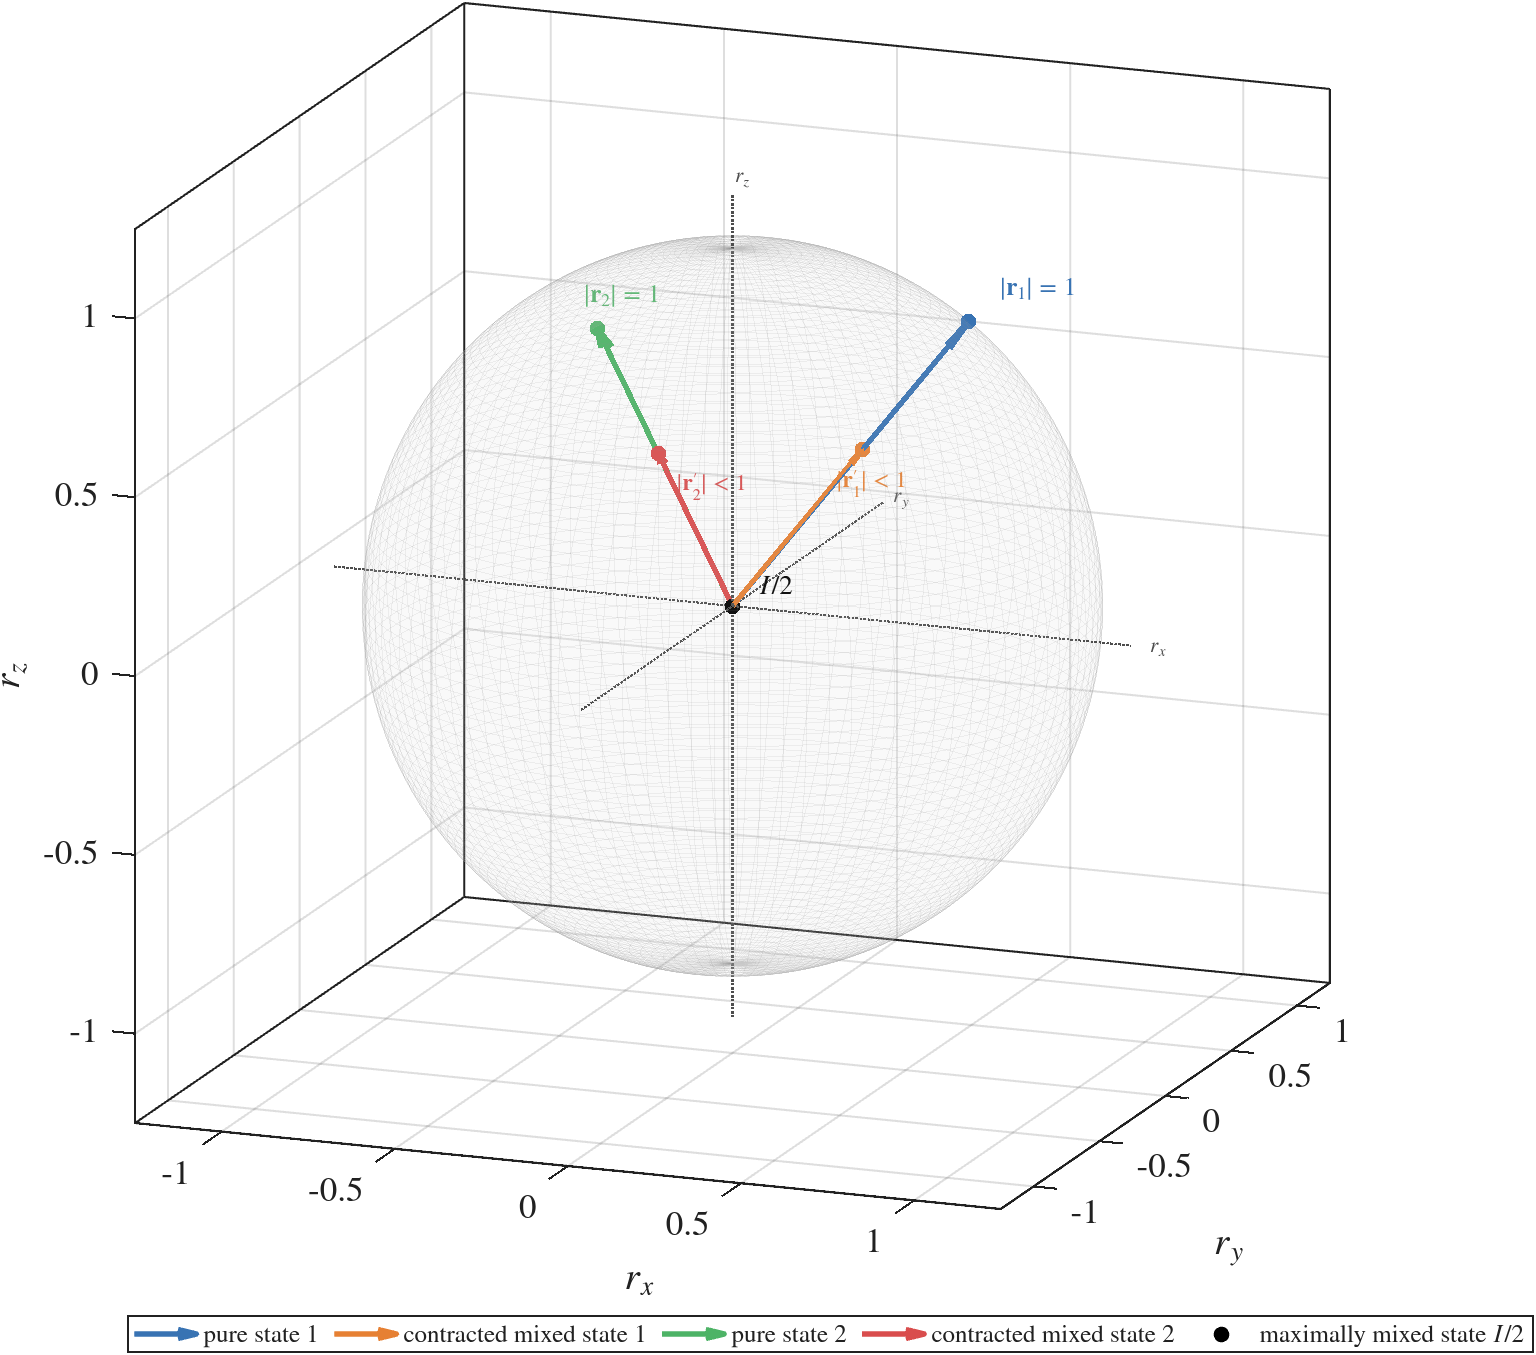
\includegraphics[
        width=0.90\textwidth
    ]{figures/theory/bloch_sphere_vector_contraction.png}
    \caption{
        Bloch-sphere representation of pure and mixed single-qubit states.
        Pure states satisfy \( \|\mathbf{r}\|=1 \), whereas mixed states are
        represented by vectors inside the Bloch sphere. The maximally mixed
        state corresponds to the origin.
    }
    \label{fig:bloch_sphere_vector_contraction}
\end{figure}

%========================================================
% SECTION 1.4 — Quantum Evolution and Quantum Channels
%========================================================

\section{Quantum Evolution and Quantum Channels}
\label{sec:quantum_evolution_channels}

The evolution of the two polarization qubits can occur either coherently or through
an effective noisy process. These two regimes are naturally distinguished within
the density-operator formalism.

%--------------------------------------------------------
% Subsection 1.4.1 — Local Unitary Evolution
%--------------------------------------------------------

\subsection{Local Unitary Evolution}
\label{subsec:local_unitary_evolution}

When each photon undergoes a coherent polarization transformation, its evolution
is represented by a unitary operator acting on the corresponding subsystem.

If \(U_A\) and \(U_B\) denote the transformations acting on arms \(A\) and \(B\),
respectively, the pure state evolves according to

\begin{equation}
|\psi_{\mathrm{out}}\rangle
=
(U_A\otimes U_B)
|\psi_{\mathrm{in}}\rangle.
\label{eq:local_unitary_state_evolution}
\end{equation}

At the density-operator level,

\begin{equation}
\rho_{\mathrm{out}}
=
(U_A\otimes U_B)
\rho_{\mathrm{in}}
(U_A^\dagger\otimes U_B^\dagger).
\label{eq:local_unitary_density_evolution}
\end{equation}

Local unitary evolution preserves global purity and bipartite entanglement.
It may nevertheless modify the correlations observed with respect to fixed
laboratory measurement axes. This distinction between a coherent transformation
and genuine entanglement degradation is central to the fiber models developed in
Chapter~\ref{ch:02_fiber_channel_modeling}.


%--------------------------------------------------------
% Subsection 1.4.2 — Quantum Channels
%--------------------------------------------------------

\subsection{Quantum Channels}
\label{subsec:quantum_channels}

A more general transformation of a quantum state is represented by a quantum
channel,

\begin{equation}
\mathcal{E}:\rho\mapsto\mathcal{E}(\rho),
\label{eq:quantum_channel_map}
\end{equation}

which is a completely positive and trace-preserving linear map.

A general channel may be written in operator-sum form as~\cite{nielsen_chuang_qcqi,kraus1971general}

\begin{equation}
\mathcal{E}(\rho)
=
\sum_\mu
K_\mu
\rho
K_\mu^\dagger,
\qquad
\sum_\mu
K_\mu^\dagger K_\mu
=
I,
\label{eq:kraus_operator_sum}
\end{equation}

where the operators \(K_\mu\) are the Kraus operators associated with the map.

Unitary evolution is recovered as the special case containing a single Kraus
operator \(K=U\). More general channels allow the reduced state to become mixed
and are therefore required to describe decoherence, depolarization, and other
effective noise mechanisms.

The specific channel models used to represent optical-fiber propagation are
introduced in Chapter~\ref{ch:02_fiber_channel_modeling}.

%========================================================
% SECTION 1.5 — Polarization Correlations and Measurements
%========================================================

\section{Polarization Correlations and Measurements}
\label{sec:polarization_correlations_measurements}

For a bipartite polarization state, the physically relevant information is not
contained only in the statistics observed separately on arms \(A\) and \(B\), but
also in how the outcomes of measurements performed on the two photons are related.

A correlation quantifies this statistical relation. If dichotomic polarization
measurements are performed on the two arms, with outcomes
\(a,b\in\{+1,-1\}\), their correlation is defined as the expectation value of the
product of the two outcomes. A positive correlation indicates a tendency to obtain
equal outcomes, whereas a negative correlation indicates a tendency to obtain
opposite outcomes. A vanishing correlation means that the positive and negative
contributions balance for the chosen pair of measurement axes.

For measurements described by Pauli operators, these joint statistics are
conveniently represented through tensor products of local observables.


%--------------------------------------------------------
% Subsection 1.5.1 — Correlation Tensor
%--------------------------------------------------------

\subsection{Correlation Tensor}
\label{subsec:correlation_tensor}

For a two-qubit state \( \rho_{AB} \), the correlation tensor is defined by

\begin{equation}
T_{ij}
=
\mathrm{Tr}
\left[
\rho_{AB}
\left(
\sigma_i\otimes\sigma_j
\right)
\right],
\qquad
i,j\in\{x,y,z\}.
\label{eq:correlation_tensor_components}
\end{equation}

Each component \(T_{ij}\) is therefore the expectation value of the product of
the outcomes obtained when measuring polarization along axis \(i\) on photon \(A\)
and along axis \(j\) on photon \(B\). Since the corresponding measurement outcomes
are assigned the values \(\pm1\), one has

\begin{equation}
-1
\leq
T_{ij}
\leq
1.
\end{equation}

In particular, \(T_{ij}=+1\) corresponds to perfect correlation,
\(T_{ij}=-1\) to perfect anticorrelation, while intermediate values quantify
partial correlation for the selected pair of measurement settings.

Equivalently, denoting by \(P_{ab}^{(i,j)}\) the joint probability of obtaining
outcomes \(a,b\in\{+1,-1\}\) when measuring along axes \(i\) and \(j\),

\begin{equation}
T_{ij}
=
P_{++}^{(i,j)}
+
P_{--}^{(i,j)}
-
P_{+-}^{(i,j)}
-
P_{-+}^{(i,j)}.
\label{eq:correlation_from_joint_probabilities}
\end{equation}

This expression makes explicit that the correlation is determined by joint
measurement statistics rather than by the local probabilities associated with
either photon separately.

The tensor \(T\in\mathbb{R}^{3\times3}\) therefore collects the nine bipartite
Pauli correlations. A single component \(T_{ij}=0\) does not in general imply that
the two subsystems are statistically independent, since correlations may still be
present along other pairs of measurement directions.

Introducing \( \sigma_0=I \), a general two-qubit state can be expanded as

\begin{equation}
\rho_{AB}
=
\frac{1}{4}
\sum_{\mu,\nu\in\{0,x,y,z\}}
S_{\mu\nu}
\sigma_\mu\otimes\sigma_\nu,
\label{eq:two_qubit_pauli_decomposition}
\end{equation}

where

\begin{equation}
S_{\mu\nu}
=
\mathrm{Tr}
\left[
\rho_{AB}
\left(
\sigma_\mu\otimes\sigma_\nu
\right)
\right].
\label{eq:generalized_stokes_parameters}
\end{equation}

The quantities \(S_{\mu\nu}\) correspond to generalized Stokes parameters.
The terms \(S_{i0}\) and \(S_{0j}\) describe the local Bloch vectors, whereas
the \(3\times3\) block \(S_{ij}\) coincides with the correlation tensor \(T\).

This representation is particularly useful in polarization experiments because
the density operator can be reconstructed from expectation values of local Pauli
measurements, as in standard two-qubit quantum-state tomography~\cite{altepeter_james_kwiat_quantum_state_tomography}.

The reconstruction follows from the orthogonality relation

\begin{equation}
\mathrm{Tr}
\left[
(\sigma_i\otimes\sigma_j)
(\sigma_k\otimes\sigma_l)
\right]
=
4\,\delta_{ik}\delta_{jl},
\qquad
i,j,k,l\in\{0,x,y,z\}.
\label{eq:pauli_tensor_orthogonality}
\end{equation}

\medskip 

\paragraph{Experimental interpretation.}
In polarization-entangled photon experiments, the joint probabilities entering
Eq.~\eqref{eq:correlation_from_joint_probabilities} are estimated from coincidence
counts between detectors associated with the corresponding outcomes on arms \(A\)
and \(B\). A coincidence identifies two detections occurring within a prescribed
temporal window and is interpreted as originating from a single emission of photon pair.
After normalization, the measured coincidence counts provide experimental
estimates of the joint probabilities required to evaluate the polarization
correlations. The practical implementation of this procedure is discussed in 
chapter \ref{ch:04_experimental_activity}, concerning experimental activity.

%--------------------------------------------------------
% Subsection 1.5.2 — Arbitrary Local Measurement Axes
%--------------------------------------------------------

\subsection{Arbitrary Local Measurement Axes}
\label{subsec:arbitrary_measurement_axes}

A projective qubit measurement along a unit vector
\( \mathbf{n}\in\mathbb{R}^{3} \) is represented by the observable

\begin{equation}
\sigma(\mathbf{n})
=
\mathbf{n}\cdot\boldsymbol{\sigma}
=
n_x\sigma_x+n_y\sigma_y+n_z\sigma_z,
\qquad
\|\mathbf{n}\|=1.
\label{eq:measurement_operator_axis}
\end{equation}

The normalization condition ensures that the observable has eigenvalues
\( \pm1 \).

For measurement directions \( \mathbf{a} \) and \( \mathbf{b} \) on subsystems
\(A\) and \(B\), respectively, the two-photon correlation is

\begin{equation}
E(\mathbf{a},\mathbf{b})
=
\mathrm{Tr}
\left[
\rho_{AB}
\left(
\sigma(\mathbf{a})\otimes\sigma(\mathbf{b})
\right)
\right].
\label{eq:axis_correlation_trace}
\end{equation}

Using Eq.~\eqref{eq:correlation_tensor_components}, this becomes

\begin{equation}
E(\mathbf{a},\mathbf{b})
=
\mathbf{a}^{\mathsf T}
T
\mathbf{b}.
\label{eq:axis_correlation_tensor_form}
\end{equation}

The correlation tensor therefore determines the expectation value associated with
any pair of local Pauli measurement directions.

Experimentally, measurements along arbitrary axes can be realized by applying
appropriate local polarization transformations before a fixed polarization
analysis stage. This provides the connection between the abstract operator
description and the wave-plate and polarization-controller settings used in the
laboratory.

%========================================================
% SECTION 1.6 — Quantitative Characterization of the State
%========================================================

\section{Quantitative Characterization of the State}
\label{sec:quantitative_state_characterization}

No single scalar quantity completely characterizes a bipartite quantum state.
Different measures are therefore used in this work to distinguish mixedness,
proximity to a target state and entanglement.

%--------------------------------------------------------
% Subsection 1.6.1 — Purity
%--------------------------------------------------------

\subsection{Purity}
\label{subsec:purity}

The purity of a density operator is defined as

\begin{equation}
\gamma(\rho)
=
\mathrm{Tr}(\rho^2).
\label{eq:purity_definition}
\end{equation}

If \( \rho \) acts on a \(d\)-dimensional Hilbert space,

\begin{equation}
\frac{1}{d}
\leq
\gamma(\rho)
\leq
1.
\label{eq:purity_bounds}
\end{equation}

The upper bound corresponds to a pure state, whereas the lower bound is attained
by the maximally mixed state \(I_d/d\).

If

\begin{equation}
\rho
=
\sum_i
\lambda_i
|i\rangle\langle i|
\label{eq:spectral_decomposition_state}
\end{equation}

is the spectral decomposition of the state, then

\begin{equation}
\gamma(\rho)
=
\sum_i \lambda_i^2.
\label{eq:purity_spectral_decomposition}
\end{equation}

For a single qubit written in Bloch form, as \(d=2\),
Eq.~\eqref{eq:bloch_density_representation} gives

\begin{equation}
\gamma(\rho)
=
\frac{1+\|\mathbf{r}\|^2}{2},
\qquad
\text{with}
\qquad
\frac{1}{2}
\leq
\gamma(\rho)
\leq
1.
\label{eq:single_qubit_purity_bloch}
\end{equation}

For the bipartite two-qubit polarization system considered throughout this work, \(d=4\),
and therefore

\begin{equation}
\frac{1}{4}
\leq
\gamma(\rho_{AB})
\leq
1.
\label{eq:two_qubit_purity_bounds}
\end{equation}

Purity quantifies mixedness but does not identify its physical origin. A mixed
reduced state may result, for example, from tracing over an entangled subsystem,
whereas a mixed global state may arise from statistical averaging or interaction
with unresolved degrees of freedom.

%--------------------------------------------------------
% Subsection 1.6.2 — Fidelity
%--------------------------------------------------------

\subsection{Fidelity}
\label{subsec:fidelity}

Throughout this work, fidelity is defined using the squared Uhlmann convention \cite{jozsa_fidelity_1994},
for two states \( \rho \) and \( \sigma \) it is given by

\begin{equation}
F(\rho,\sigma)
=
\left[
\mathrm{Tr}
\left(
\sqrt{
\sqrt{\rho}\,
\sigma\,
\sqrt{\rho}
}
\right)
\right]^2.
\label{eq:fidelity_general_definition}
\end{equation}

When the reference state is pure,
\( \sigma=|\phi\rangle\langle\phi| \), the expression simplifies to

\begin{equation}
F(\rho,|\phi\rangle)
=
\langle\phi|\rho|\phi\rangle.
\label{eq:fidelity_pure_reference}
\end{equation}

In this thesis the principal reference is \( |\Psi^+\rangle \), so that

\begin{equation}
F_{\Psi^+}
=
\langle\Psi^+|\rho|\Psi^+\rangle.
\label{eq:fidelity_psi_plus_definition}
\end{equation}

Fidelity measures similarity to a chosen target and must therefore not be
interpreted directly as an entanglement measure. A local unitary transformation
can substantially change \(F_{\Psi^+}\) while leaving the amount of entanglement
unchanged.

%--------------------------------------------------------
% Subsection 1.6.3 — Concurrence and Tangle
%--------------------------------------------------------

\subsection{Concurrence and Tangle}
\label{subsec:concurrence_tangle}

The qualitative distinction between separable and entangled states was introduced
in Section~\ref{sec:reference_entangled_state}. A quantitative measure is now
required to characterize the degree of entanglement of the propagated two-qubit
state. Throughout this work, concurrence is adopted as the principal measure of
bipartite entanglement~\cite{wootters_entanglement_1998}.

For a pure state

\begin{equation}
|\psi\rangle
=
a|00\rangle
+b|01\rangle
+c|10\rangle
+d|11\rangle,
\label{eq:general_pure_two_qubit_state_concurrence}
\end{equation}

the concurrence is

\begin{equation}
C(|\psi\rangle)
=
2|ad-bc|.
\label{eq:pure_state_concurrence}
\end{equation}

It satisfies

\begin{equation}
0\leq C\leq1,
\end{equation}

with \(C=0\) for separable pure states and \(C=1\) for maximally entangled
two-qubit states.

For pure bipartite states, concurrence can also be expressed through either
reduced density operator,

\begin{align}
C(|\psi_{AB}\rangle)
&=
2\sqrt{\det\rho_A}
=
\sqrt{
2\left[
1-\mathrm{Tr}(\rho_A^2)
\right]
}
\nonumber
\\
&=
2\sqrt{\det\rho_B}
=
\sqrt{
2\left[
1-\mathrm{Tr}(\rho_B^2)
\right]
}.
\label{eq:concurrence_reduced_density_relation}
\end{align}

The equivalence follows from the fact that, for a globally pure bipartite state,
\(\rho_A\) and \(\rho_B\) have the same nonzero eigenvalues.

For a mixed two-qubit state, concurrence is defined through the Wootters
spin-flip construction~\cite{wootters_entanglement_1998}. Defining

\begin{equation}
\widetilde{\rho}
=
(\sigma_y\otimes\sigma_y)
\rho^*
(\sigma_y\otimes\sigma_y),
\label{eq:spin_flipped_density_matrix}
\end{equation}

and denoting by
\(\lambda_1\geq\lambda_2\geq\lambda_3\geq\lambda_4\)
the square roots of the eigenvalues of
\(\rho\widetilde{\rho}\), one obtains

\begin{equation}
C(\rho)
=
\max
\left(
0,\,
\lambda_1-\lambda_2-\lambda_3-\lambda_4
\right).
\label{eq:mixed_state_concurrence}
\end{equation}

The associated tangle is defined as

\begin{equation}
\tau(\rho)
=
C(\rho)^2.
\label{eq:tangle_definition}
\end{equation}

For the reference Bell state,

\begin{equation}
C(|\Psi^+\rangle)=1,
\qquad
\tau(|\Psi^+\rangle)=1.
\end{equation}

Both quantities are invariant under local unitary transformations, consistently
with the invariance of bipartite entanglement under local changes of polarization
basis.

%--------------------------------------------------------
% Subsection 1.6.4 — Entanglement of Formation
%--------------------------------------------------------

\subsection{Entanglement of Formation}
\label{subsec:entanglement_of_formation}

The entanglement of formation provides a resource-oriented measure of bipartite
entanglement. For two qubits, it can be expressed analytically in terms of the
concurrence~\cite{wootters_entanglement_1998} as

\begin{equation}
E_F(\rho)
=
h
\left(
\frac{
1+\sqrt{1-C(\rho)^2}
}{2}
\right),
\label{eq:eof_definition}
\end{equation}

where

\begin{equation}
h(x)
=
-x\log_2x
-
(1-x)\log_2(1-x)
\label{eq:binary_entropy_function}
\end{equation}

is the binary entropy.

For two-qubit states,

\begin{equation}
0\leq E_F\leq1,
\end{equation}

with \(E_F=0\) for separable states and \(E_F=1\) for maximally entangled
Bell states. Because \(E_F\) is a monotonic function of concurrence for
two-qubit states, the two quantities preserve the same ordering of entanglement,
while providing different quantitative representations.

%========================================================
% SECTION 1.7 — Complementarity of the State Metrics
%========================================================

\section{Complementarity of the State Metrics}
\label{sec:complementarity_state_metrics}

The quantities introduced in the previous sections characterize different
properties of the same density operator and should therefore not be interpreted
interchangeably. Purity quantifies whether a state is pure or mixed but does not
measure entanglement, while fidelity quantifies similarity with respect to a
selected reference state and can change under coherent local transformations.
Concurrence, tangle, and entanglement of formation instead quantify bipartite
entanglement.

This distinction is particularly relevant for optical-fiber propagation. A
coherent local polarization transformation may alter the correlations measured
along fixed laboratory axes and reduce fidelity with respect to the initial Bell
state without changing purity or entanglement. By contrast, unresolved
statistical fluctuations or coupling between polarization and unobserved degrees
of freedom may produce mixedness and a reduction of the distributed
entanglement.

The simultaneous evaluation of these quantities therefore provides a
state-level description capable of distinguishing coherent transformations from
decoherence and entanglement degradation. Their operational significance,
however, depends on the application for which the distributed state is intended.
For this reason, the following section introduces the BBM92 protocol and the
quantities used in this work to connect the characterization of the quantum state
with the requirements of entanglement-based quantum communication.

%========================================================
% SECTION 1.8 — BBM92 and Operational Requirements
%========================================================

\section{BBM92 and Operational Requirements}

\label{sec:bbm92_operational_requirements}

The main operational reference considered in this thesis is the BBM92 entanglement-based
quantum key distribution protocol~\cite{bennett_brassard_mermin_BBM92_1992}.
In its polarization implementation, a source distributes the two photons of an entangled
pair to two spatially separated parties, conventionally denoted Alice and Bob. Each party
independently selects between alternative polarization measurement bases. Measurements
performed using compatible bases provide correlated outcomes that can be used for key
generation and for estimating the disturbance introduced along the communication link.

A conceptual representation of the polarization-encoded BBM92 architecture adopted as
operational reference throughout this work is shown in
Fig.~\ref{fig:bbm92_reference_architecture}.

\begin{figure}[htbp]
    \centering

    \resizebox{0.95\textwidth}{!}{%
    \begin{tikzpicture}[
        >=Latex,
        line width=0.8pt,
        font=\small,
        source/.style={
            draw,
            rectangle,
            rounded corners=1pt,
            minimum width=4.2cm,
            minimum height=0.8cm,
            align=center
        },
        bs/.style={
            draw,
            fill=blue!20,
            minimum width=0.16cm,
            minimum height=0.85cm,
            rotate=45
        },
        hwp/.style={
            draw,
            fill=blue!20,
            minimum width=0.75cm,
            minimum height=0.16cm
        },
        pbs/.style={
            draw,
            fill=blue!8,
            minimum width=0.70cm,
            minimum height=0.70cm,
            path picture={
                \draw
                (path picture bounding box.south west)
                --
                (path picture bounding box.north east);
            }
        },
        detector/.style={
            draw,
            rounded corners=3pt,
            fill=blue!15,
            minimum width=1.20cm,
            minimum height=0.55cm,
            align=center
        },
        link/.style={
            -{Latex[length=2mm]}
        }
    ]

    %----------------------------------------------------
    % Entangled-photon source
    %----------------------------------------------------

    \node[source] (source) at (0,5.7)
    {Entangled Photons Source};

    %----------------------------------------------------
    % Alice
    %----------------------------------------------------

    \node[bs] (aBS) at (-3.5,4.0) {};

    % Z-basis branch
    \node[pbs] (aPBSZ) at (-5.6,4.0) {};
    \node[detector] (aH) at (-7.5,4.0) {SPAD$_H$};
    \node[detector] (aV) at (-5.6,2.8) {SPAD$_V$};

    % X-basis branch
    \node[hwp] (aHWP) at (-3.5,3.15) {};
    \node[pbs] (aPBSX) at (-3.5,2.00) {};
    \node[detector] (aD) at (-1.8,2.00) {SPAD$_D$};
    \node[detector] (aA) at (-3.5,0.80) {SPAD$_A$};

    % Alice optical paths
    \draw[link]
    (source.south west)
    --
    (aBS);

    \draw
    (aBS)
    --
    node[above, font=\scriptsize]
    {\(Z\) basis}
    (aPBSZ);

    \draw[link]
    (aPBSZ)
    --
    (aH);

    \draw[link]
    (aPBSZ)
    --
    (aV);

    \draw
    (aBS)
    --
    (aHWP);

    \draw
    (aHWP)
    --
    node[right, font=\scriptsize]
    {\(X\) basis}
    (aPBSX);

    \draw[link]
    (aPBSX)
    --
    (aD);

    \draw[link]
    (aPBSX)
    --
    (aA);

    % Labels
    \node[font=\scriptsize, right=1mm of aBS]
    {50:50 BS};

    \node[font=\scriptsize, right=1mm of aHWP]
    {HWP \(22.5^\circ\)};

    \node[font=\scriptsize, above=1mm of aPBSZ]
    {PBS};

    \node[font=\scriptsize, left=1mm of aPBSX]
    {PBS};

    % Alice box
    \node[
        draw,
        dashed,
        rounded corners,
        fit=(aBS)(aPBSZ)(aH)(aV)(aHWP)(aPBSX)(aD)(aA),
        inner sep=6mm,
        label={[font=\bfseries]above:Alice}
    ] {};

    %----------------------------------------------------
    % Bob — specular configuration with respect to Alice
    %----------------------------------------------------

    \node[bs] (bBS) at (3.5,4.0) {};

    % Z-basis branch
    \node[pbs] (bPBSZ) at (5.6,4.0) {};
    \node[detector] (bH) at (7.5,4.0) {SPAD$_H$};
    \node[detector] (bV) at (5.6,2.8) {SPAD$_V$};

    % X-basis branch
    \node[hwp] (bHWP) at (3.5,3.15) {};
    \node[pbs] (bPBSX) at (3.5,2.00) {};
    \node[detector] (bD) at (1.8,2.00) {SPAD$_D$};
    \node[detector] (bA) at (3.5,0.80) {SPAD$_A$};

    % Bob optical paths
    \draw[link]
    (source.south east)
    --
    (bBS);

    \draw
    (bBS)
    --
    node[above, font=\scriptsize]
    {\(Z\) basis}
    (bPBSZ);

    \draw[link]
    (bPBSZ)
    --
    (bH);

    \draw[link]
    (bPBSZ)
    --
    (bV);

    \draw
    (bBS)
    --
    (bHWP);

    \draw
    (bHWP)
    --
    node[left, font=\scriptsize]
    {\(X\) basis}
    (bPBSX);

    \draw[link]
    (bPBSX)
    --
    (bD);

    \draw[link]
    (bPBSX)
    --
    (bA);

    % Labels
    \node[font=\scriptsize, left=1mm of bBS]
    {50:50 BS};

    \node[font=\scriptsize, left=1mm of bHWP]
    {HWP \(22.5^\circ\)};

    \node[font=\scriptsize, above=1mm of bPBSZ]
    {PBS};

    \node[font=\scriptsize, right=1mm of bPBSX]
    {PBS};

    % Bob box
    \node[
        draw,
        dashed,
        rounded corners,
        fit=(bBS)(bPBSZ)(bH)(bV)(bHWP)(bPBSX)(bD)(bA),
        inner sep=6mm,
        label={[font=\bfseries]above:Bob}
    ] {};

    \end{tikzpicture}
    }

    \caption{
    Conceptual polarization-encoded BBM92 architecture used as the operational
    reference in this work. The entangled-photon source distributes one photon
    through fiber arm \(A\) to Alice and the second through fiber arm \(B\) to
    Bob. At each receiver, a 50:50 beam splitter (BS) provides passive basis
    selection. The direct polarization beam splitter (PBS) analyzes the
    computational \(Z=\{H,V\}\) basis, whereas a half-wave plate (HWP) followed
    by a PBS enables measurement in the diagonal \(X=\{D,A\}\) basis.
    The resulting polarization components are detected by single-photon
    avalanche diodes (SPADs).
    }
    \label{fig:bbm92_reference_architecture}

\end{figure}

For the polarization encoding adopted throughout this work, the computational
basis has already been identified with
\begin{equation}
|0\rangle\equiv|H\rangle,
\qquad
|1\rangle\equiv|V\rangle,
\nonumber
\end{equation}
while the complementary diagonal basis is
\begin{equation}
|D\rangle
=
\frac{|H\rangle+|V\rangle}{\sqrt{2}},
\qquad
|A\rangle
=
\frac{|H\rangle-|V\rangle}{\sqrt{2}}.
\label{eq:bbm92_diagonal_basis}
\end{equation}

For an ideal entangled state, Alice and Bob obtain the expected correlations in both measurement bases. Propagation through the optical link may modify these correlations and introduce errors. Their magnitude is described by the basis-dependent quantum bit error rates
\begin{equation}
Q_Z,
\qquad
Q_X,
\label{eq:bbm92_basis_qber}
\end{equation}
associated with measurements in the computational and diagonal bases, respectively. These quantities can be obtained from the joint measurement probabilities of the propagated two-photon state.

The QBER provides the first operational connection between the quantum state distributed through the fiber and the BBM92 protocol. Degradation or misalignment of the expected polarization correlations increases the measured error rates and therefore increases the amount of information that must be removed during the classical post-processing stages required to obtain a secure key. However, QBER alone does not quantify the rate at which secure key bits can ultimately be generated. A complete protocol-level characterization is instead provided by the Secure Key Rate (SKR), which combines the quality of the measured correlations with the detected coincidence rate and the classical costs associated with error correction and privacy amplification.

In the asymptotic BBM92 description~\cite{dinardo_thesis}, the secure key rate can be expressed in the general form
\begin{equation}
R_{\mathrm{SK}}
=
q\,R_{\mathrm{cc}}
\left[
1
-
f(E_{\mathrm{bit}})
H_2(E_{\mathrm{bit}})
-
H_2(E_{\mathrm{ph}})
\right],
\label{eq:bbm92_skr_general}
\end{equation}
where \(R_{\mathrm{cc}}\) denotes the measured coincidence rate, \(q\) is the basis-sifting factor, \(f(E_{\mathrm{bit}})\geq1\) accounts for the inefficiency of practical error-correction procedures, and
\begin{equation}
H_2(x)
=
-x\log_2x
-
(1-x)\log_2(1-x)
\label{eq:binary_entropy_bbm92}
\end{equation}
is the binary entropy. The quantity \(E_{\mathrm{bit}}\) represents the error rate associated with the basis used for key generation, whereas \(E_{\mathrm{ph}}\) represents the corresponding phase-error rate inferred from measurements in the complementary basis.

For example, when the \(Z\) basis is used for key generation, one may identify
\begin{equation}
E_{\mathrm{bit}}=Q_Z,
\qquad
E_{\mathrm{ph}}=Q_X.
\label{eq:bbm92_bit_phase_errors}
\end{equation}
The roles are exchanged if the \(X\) basis is instead used for key generation. In the symmetric case \(Q_Z=Q_X=Q\), Eq.~\eqref{eq:bbm92_skr_general} reduces to
\begin{equation}
R_{\mathrm{SK}}
=
q\,R_{\mathrm{cc}}
\left[
1
-
\left(
1+f(Q)
\right)
H_2(Q)
\right].
\label{eq:bbm92_skr_symmetric}
\end{equation}

Equation~\eqref{eq:bbm92_skr_general} clarifies the distinction between the different modeling levels considered in this thesis. The propagated density operator determines the ideal polarization measurement probabilities and therefore the state-induced contributions to \(Q_Z\) and \(Q_X\). The complete experimentally achievable SKR additionally depends on quantities that are not determined by the polarization density operator alone, such as source brightness, optical transmission losses, detector efficiencies, dark-count rates, timing jitter, the coincidence-window duration, and the adopted classical post-processing scheme. These additional contributions are therefore treated as system-level parameters rather than intrinsic properties of the propagated quantum state.

The objective of this work is consequently not only to quantify degradation of the distributed entanglement, but also to determine which physical configurations of the optical link remain compatible with useful BBM92 operation. For this purpose, the physical configuration is represented by the parameter vector
\begin{equation}
\boldsymbol{\xi}
=
\{
\xi_1,\xi_2,\ldots,\xi_m
\},
\label{eq:physical_parameter_vector}
\end{equation}
which collects the relevant source and fiber parameters. Depending on the model, these may include photon spectral bandwidth, spectral correlation, differential group delay, birefringence orientation, and compensation parameters.

For each physical configuration \(\boldsymbol{\xi}\), the propagated state is characterized by a corresponding set of quantities
\begin{equation}
\boldsymbol{\lambda}(\boldsymbol{\xi})
=
\{
\gamma,\,
F,\,
C,\,
Q_Z,\,
Q_X,\,
\ldots
\},
\label{eq:state_metric_vector}
\end{equation}
where \(\gamma\), \(F\), and \(C\) characterize the state in terms of mixedness, similarity to the reference state, and entanglement, while \(Q_Z\) and \(Q_X\) provide the direct interface with the BBM92 security analysis.

The relation between the physical fiber model, the resulting state, and the protocol-level performance can therefore be summarized as
\begin{equation}
\boxed{
\boldsymbol{\xi}
\longrightarrow
\rho_{AB}(\boldsymbol{\xi})
\longrightarrow
\boldsymbol{\lambda}(\boldsymbol{\xi})
\longrightarrow
R_{\mathrm{SK}}
}
\label{eq:physical_to_operational_mapping}
\end{equation}
where the final step additionally depends on the remaining source, detection, and post-processing parameters required by the complete BBM92 system model.

A first operational region can be defined directly from the QBER by requiring the relevant error quantities to remain below an adopted security threshold \(Q_{\mathrm{th}}\),
\begin{equation}
\mathcal{R}_{Q}
=
\left\{
\boldsymbol{\xi}
:
Q_Z(\boldsymbol{\xi})<Q_{\mathrm{th}},
\;
Q_X(\boldsymbol{\xi})<Q_{\mathrm{th}}
\right\}.
\label{eq:bbm92_qber_operating_region}
\end{equation}
Here, \(Q_{\mathrm{th}}\) is not an arbitrary state-quality threshold, but follows from the adopted security model and post-processing assumptions.

At the complete system level, a more direct definition of useful BBM92 operation is obtained from the condition that a positive secure key rate can be extracted,
\begin{equation}
\boxed{
\mathcal{R}_{\mathrm{BBM92}}
=
\left\{
\boldsymbol{\xi}
:
R_{\mathrm{SK}}(\boldsymbol{\xi})>0
\right\}.
}
\label{eq:bbm92_operating_region}
\end{equation}
More restrictive requirements may be introduced when a minimum useful key throughput \(R_{\mathrm{SK,th}}>0\) is required for a specific application.

Concurrence plays a complementary role in this analysis. It provides a compact measure of the surviving bipartite entanglement and is therefore used extensively to characterize the effect of fiber propagation. However, concurrence, QBER, and SKR quantify different properties and are not generally equivalent. In particular, a coherent polarization rotation may change the QBER measured in fixed bases without changing the amount of entanglement, while two systems producing the same quantum state and the same QBER may yield very different secure key rates because of different optical losses, detector efficiencies, dark counts, or coincidence rates.

For this reason, a universal concurrence threshold for BBM92 operation is not assumed. Instead, the numerical analysis investigates how concurrence and the basis-dependent QBERs vary together for the specific families of states produced by the considered fiber models. When a clear correspondence exists for a particular model, an operational QBER boundary can then be associated with a corresponding value of concurrence. The subsequent inclusion of the remaining experimental parameters allows the same framework to be extended from state-quality maps to SKR-based communication-performance maps.

The resulting hierarchy has a direct practical interpretation: \(\boldsymbol{\xi}\) describes the physical source and fiber configuration, \(\rho_{AB}\) describes the resulting distributed quantum state, \(\boldsymbol{\lambda}\) contains its state-quality and QBER diagnostics, and \(R_{\mathrm{SK}}\) quantifies the final secure-key throughput once the complete source, link, detector, and post-processing model is specified. This perspective is used in Chapter~\ref{ch:03_numerical_simulations_results} to construct operational maps and investigate how the boundaries of useful entanglement distribution depend on the physical parameters of the optical link.

%========================================================
% END OF CHAPTER 1
%========================================================